\documentclass[preprint,10pt,authoryear]{elsarticle}
\usepackage[UTF8]{ctex}
\usepackage{amssymb}
\usepackage{amsmath}
\usepackage{xcolor}

\usepackage{geometry}
\geometry{
  top=1in,
  bottom=1in,
  left=0.7in,
  right=0.7in
}

\usepackage{graphicx} 
\usepackage{subcaption}  

\usepackage{xspace}

\usepackage{hyperref}
\hypersetup{
    colorlinks=true,
    linkcolor=blue,
    urlcolor=blue,
    citecolor=blue
}

\usepackage[capitalize,nameinlink]{cleveref}
\crefname{section}{节}{节}
\Crefname{section}{节}{节}
\crefname{table}{表}{表}
\Crefname{table}{表}{表}
\crefname{figure}{图}{图}
\Crefname{figure}{图}{图}
\crefname{equation}{式}{式}
\Crefname{equation}{式}{式}
\crefname{algorithm}{算法}{算法}
\Crefname{algorithm}{算法}{算法}

\usepackage{caption}   
\DeclareCaptionLabelFormat{myformat}{\textbf{图 #2}}
\captionsetup[figure]{labelformat=myformat}


\usepackage{multirow} 
\usepackage{algorithm}  
\usepackage{algpseudocode}  
% \usepackage{caption}   
\usepackage{booktabs} 
\usepackage{setspace}  
\usepackage{lineno}
\modulolinenumbers[1]

\newcommand{\METHOD}{TopoWheat\xspace}
\newcommand{\TRPL}{TRPL\xspace}
\newcommand{\TRPLfull}{Topology-Reliable Pseudo-Labeling\xspace}
\newcommand{\TCPM}{TCPM\xspace}
\newcommand{\TCPMfull}{Topology-Core Prototype Memory\xspace}
\newcommand{\BAZR}{BAZR\xspace}
\newcommand{\BAZRfull}{Break-Aware Zoom Refinement\xspace}
\newcommand{\placeholder}[1]{%
  \ifmmode
    \text{\textcolor{blue}{【#1】}}%
  \else
    \textcolor{blue}{【#1】}%
  \fi
}

\DeclareRobustCommand{\rev}[2]{%
  \ifcase#1%
    #2%
  \or%
    \textcolor{blue}{#2}%
  \or%
    \textcolor{red}{#2}%
  \else%
    #2%
  \fi%
}

\begin{document}
\linenumbers

\begin{frontmatter}
\title{\METHOD：面向跨域小样本小麦器官分割的拓扑可靠半监督学习与断裂感知精细化方法}
\author[1,2]{Yiqun Wang}
\author[1,2]{Shuo Zhang}
% \author[1,2]{Xiaolong Liu}
\author[3,4]{Ze Ji}
% \author[3]{Guoliang Liu}
\author[1,2]{Weikuan Jia\corref{co}}
\cortext[co]{Corresponding author.}
% \affiliation[1]{School of Computer Science and Artificial Intelligence, Shandong Normal University, Jinan 250358, China}
\affiliation[1]{
    organization={School of Computer Science and Artificial Intelligence, Shandong Normal University},
    city={Jinan 250358},
    % postcode={},
    country={China},
}
\affiliation[2]{
    organization={Shandong Key Laboratory of Intelligent Collaborative Perception and Computing, Shandong Normal University},
    city={Jinan 250358},
    % postcode={},
    country={China},
}
\affiliation[3]{
    organization={College of Mechanical and Electrical Engineering, Hohai University},
    city={Changzhou 213200},
    % postcode={},
    country={China},
}
\affiliation[4]{
    organization={School of Engineering, Cardiff University},
    city={Cardiff CF24 3AA},
    % postcode={},
    country={United Kingdom},
}

\begin{abstract}
复杂田间环境中的小麦器官语义分割是解析群体结构、器官比例及生育进程的重要基础，但其性能受到像素级标注稀缺、采集域差异以及细长茎秆易断裂等因素的共同制约。现有半监督方法通常依据区域或像素置信度筛选伪标签，难以区分茎秆中心线的结构可靠性与边界宽度的不确定性；现有跨域方法也容易将噪声边界引入类别对齐。高精度方案依赖的密集多尺度滑窗还会带来显著计算开销。针对这些相互关联的问题，本文提出统一框架 \METHOD。框架中的拓扑可靠伪标签学习模块 \TRPL 利用多尺度与扰动一致性，将无标注茎秆监督解耦为稳定中心线、可靠区域和不确定边界。由此获得的稳定结构不只服务于伪监督，还被拓扑核心原型记忆模块 \TCPM 用来构建域级和全局类别原型，通过留一域模拟与对比约束学习域不变器官表示。推理时，断裂感知选择性放大模块 \BAZR 复用同一拓扑线索，根据茎秆预测熵、骨架端点和内部尺度分歧定位困难区域，仅对少量候选窗口执行高分辨率精细化。在 GWFSS 少标注协议和完整数据地域协议上，\METHOD 取得了 \placeholder{XX.XX\%} 的验证 mIoU 和 \placeholder{XX.XX\%} 的未知域测试 mIoU，茎秆 IoU 较统一主干监督基线提高 \placeholder{X.XX} 个百分点。与密集多尺度推理相比，所提方法将分割器前向次数从约 160 次降至 5 次，同时保持了竞争性的分割精度。
\end{abstract}

\begin{keyword}
小麦器官分割，半监督语义分割，拓扑可靠伪标签，域泛化，高分辨率精细化
\end{keyword}

\end{frontmatter}

%%%%%%%%% BODY TEXT
% STATUS: QUARANTINED old-method narrative; see ../METHOD_STATUS.md.
\section{引言}
\label{sec:introduction}

小麦器官的数量、空间分布、颜色变化和衰老进程与冠层结构、生长状态及产量形成密切相关 \citep{li2021canopy,li2021lai,dandrifosse2022ear}。高空间分辨率 RGB 成像为这些性状提供了低成本、非破坏性的田间测量手段，但可靠测量仍依赖对麦穗、叶片、茎秆和背景的准确区分。与以麦穗定位为目标的检测任务不同，器官级语义分割必须同时处理叶片交叠、茎秆遮挡、组织衰老、杂草干扰和土壤残体等复杂因素。GWFSS 数据集覆盖多个国家、研究机构、生育期和成像平台，为研究真实田间条件下的小麦器官分割提供了统一基础 \citep{wang2025gwfss}。

困难并不只来自训练样本数量。少标注协议仅提供 99 张像素级标注图像，而无标注图像超过六万张，教师模型生成的伪标签因而承担了大量监督作用。细茎只占少量像素，其边界置信度又显著低于叶片和背景；固定阈值往往把整个不确定掩码删除，使中心位置正确、宽度尚不确定的茎秆监督也随之消失。采集条件的变化进一步放大了这种偏差。不同机构的图像在光照、基因型、生育期、相机视角和地面采样距离上存在明显差异，地域划分下显著低于随机划分的结果表明，未知采集域泛化是实际部署中的核心障碍 \citep{wang2025gwfss}。分辨率则构成另一层制约：放大输入确实有助于识别细茎，但密集覆盖多个尺度会对同一区域反复计算 \citep{cao2025detailminority}，难以满足高通量表型分析的效率要求。

现有研究分别从半监督学习、结构保持和跨域表示等角度缓解上述问题。Mean Teacher 及其后续方法使用指数滑动平均教师为学生提供稳定监督 \citep{tarvainen2017mean,berrada2024guided}；UniMatch、U2PL 和 ST++ 分别从强弱扰动、不可靠像素利用和样本稳定性角度改进伪标签学习 \citep{yang2023unimatch,wang2022u2pl,yang2022stpp}。然而，这些方法主要依据像素、区域或图像层面的置信度处理噪声，没有针对细长器官区分结构位置与边界宽度的不确定性。soft-clDice 等方法能够增强管状目标的拓扑连续性 \citep{shit2021cldice}，但直接将拓扑损失作用于噪声伪标签可能强化错误连接。域泛化方法通过类别记忆或域间对齐学习稳定表示 \citep{kim2022pinmemory}，由全部预测像素构建的原型仍会受到细茎边界噪声污染。

稀缺标注条件下的跨域细茎分割不宜被拆成彼此独立的伪标签筛选、域对齐和高分辨率推理问题。伪标签中稳定的拓扑核心能够为跨域原型提供较干净的语义依据，同一结构表示也能够指示哪些局部区域真正需要更高分辨率。沿着这条信息路径，本文构建了 \METHOD。基础分割器由 BEiTv2-Large、ViT-Adapter 和 Mask2Former 组成 \citep{peng2022beitv2,chen2023vitadapter,cheng2022mask2former}，其教师--学生训练过程同时建立拓扑可靠伪监督和跨域器官原型，推理过程则利用预测中的结构失效信号分配局部计算。

\METHOD 的主要贡献不是简单叠加三个独立部件，而是让拓扑可靠性在训练和推理之间发挥一致作用。\TRPL 通过多尺度与扰动一致性估计，将茎秆监督表示为稳定中心线、可靠区域和不确定边界，避免固定阈值整体丢弃细结构。\TCPM 接收这一稳定核心，以课程日程依次建立有标注和高质量伪标注类别--域记忆，并用逐样本留一域锚点校正可靠区域中偏移最明显的困难特征，使干净的原型来源与有效的梯度位置彼此分离。\BAZR 进一步把结构不确定性转化为推理预算，根据预测熵、骨架端点和内部尺度分歧选择少量高分辨率窗口。少标注跨域评测、完整数据地域划分、针对性消融和精度--效率分析共同验证了这一设计链路。


\section{相关工作}
\label{sec:related-work}

\subsection{标注稀缺条件下的器官分割}

早期田间作物分割通常依赖颜色指数或卷积编码器--解码器。DeepLabV3+ 通过空洞卷积和低层特征融合兼顾上下文与边界 \citep{chen2018deeplabv3plus}，SegFormer 则使用层次化 Transformer 和轻量解码器获得更强的全局建模能力 \citep{xie2021segformer}。GWFSS 数据集上的比较表明，SegFormer 在随机划分和区域划分下均优于 DeepLabV3+，但茎秆仍明显弱于其他器官 \citep{wang2025gwfss}。Mask2Former 将语义分割统一为类别查询与掩码预测问题 \citep{cheng2022mask2former}，ViT-Adapter 则使预训练视觉 Transformer 能够输出适合密集预测的多尺度特征 \citep{chen2023vitadapter}。

有限标注使单纯监督训练容易过拟合。Mean Teacher 使用学生参数的指数滑动平均构建教师 \citep{tarvainen2017mean}，Guided Distillation 进一步在学生预热阶段同时使用有标注与无标注数据 \citep{berrada2024guided}。弱到强一致性方法通过教师的弱扰动预测监督学生的强扰动视图，已成为半监督语义分割的重要范式 \citep{yang2023unimatch}。ST++ 使用跨训练阶段的预测稳定性选择可靠图像 \citep{yang2022stpp}，U2PL 则将不可靠像素作为负类监督以减少无标注信息浪费 \citep{wang2022u2pl}。在小麦器官分割中，已有方法进一步使用器官比例或特征相似度选择无标注图像，并利用不确定性过滤伪标签 \citep{cao2025detailminority,ghosh2025decon}。这些方法提高了无标注数据利用率，但仍将茎秆伪标签主要视为普通区域，没有显式区分中心线结构与宽度边界的可靠性。

\subsection{细长器官的结构完整性}

茎秆具有占比低、宽度小、遮挡频繁和方向连续等特点。低分辨率特征与常规插值容易模糊其边界，PointRend 因而将不确定边界位置视为需要进一步渲染的点 \citep{kirillov2020pointrend}。这类局部细化能够恢复边界细节，但没有直接约束细长目标的连续性。

拓扑保持损失为管状结构分割提供了另一种思路。soft-clDice 通过预测掩码与参考掩码骨架之间的重合关系度量拓扑精度和拓扑召回率 \citep{shit2021cldice}；中心线交叉熵进一步讨论了拓扑一致性与区域精度之间的平衡 \citep{acebes2024clce}。近期工作还从深浅层特征融合和生长--抑制平衡角度增强不同宽度管状结构的识别 \citep{huang2025harmonyseg}。然而，小麦茎秆并不等同于完整可见的血管或道路，其真实标注可能因叶片遮挡而中断。直接对所有预测强制连通会产生不符合可见区域定义的虚假连接。因此，本文只在多视图一致的可见中心线上施加拓扑监督，并将不可靠边界保留为忽略区域。

\subsection{未知采集域中的器官语义稳定性}

田间图像的域差异同时来自成像设备、光照、背景、基因型和生育阶段。GWFSS 的特征可视化呈现出明显的机构聚类，区域划分下的性能下降也说明随机划分难以反映真实部署难度 \citep{wang2025gwfss}。域泛化语义分割要求训练阶段不访问目标域，学习能够迁移到未知环境的表示 \citep{schwonberg2025dgsurvey}。类别记忆方法通过元学习保存跨域共享的类别模式 \citep{kim2022pinmemory}，多分辨率域适应方法则表明全局上下文与高分辨率局部信息对小目标和跨域鲁棒性均有价值 \citep{hoyer2022hrda}。

对小麦器官而言，不同类别的域稳定区域并不相同。叶片和背景具有较大的内部区域，而茎秆最可靠的位置通常位于细长结构的中心。现有类别原型通常从全部预测像素或置信区域求均值，仍可能受到边界混淆和伪标签噪声影响；在半监督早期把人工标注与伪标注写入同一记忆，还会使错误类别中心持续影响后续特征。本文从拓扑核心而非完整预测区域构建域级原型，以课程式双记忆隔离两类证据，并在读取参照时对每个样本排除其自身域，以减小未知地域上的语义漂移。

\subsection{高分辨率细化的精度与效率}

将图像放大后进行滑窗预测能够提升小目标和细结构的可见尺度。SAHI 通过切片推理增强小目标检测 \citep{akyon2022sahi}，高分辨率域适应方法利用低分辨率全局图像和高分辨率局部裁剪融合上下文与细节 \citep{hoyer2022hrda}。GWFSS 上的多尺度滑窗策略证明了放大输入对茎秆分割的有效性，但密集覆盖多个尺度会产生较高推理开销 \citep{cao2025detailminority}。SparseRefine 使用预测熵选择少量高分辨率像素进行稀疏修正 \citep{liu2024sparserefine}，说明选择性计算是提高高分辨率分割效率的可行方向。

单纯的熵能够定位分类不确定区域，却不能区分普通纹理边界与影响茎秆完整性的结构失效。本文进一步联合茎秆概率、异常骨架端点和跨尺度断裂程度评价候选窗口，使高分辨率计算优先服务于细长器官的真实困难区域。


% STATUS: QUARANTINED. The mechanisms below failed their matched controls.
% See ../METHOD_STATUS.md and ../../METHOD_REDESIGN.md.
\section{方法}
\label{sec:method}

\subsection{问题定义}

设有标注数据集为
\begin{equation}
\mathcal D_l=\{(x_i^l,y_i^l,d_i)\}_{i=1}^{N_l},
\end{equation}
其中 $x_i^l\in\mathbb R^{3\times H\times W}$ 表示田间 RGB 图像，$y_i^l\in\{0,\ldots,C-1\}^{H\times W}$ 表示像素级标注，$d_i\in\{1,\ldots,D\}$ 表示采集域。无标注数据集记为
\begin{equation}
\mathcal D_u=\{(x_j^u,d_j)\}_{j=1}^{N_u}.
\end{equation}
本文考虑背景、麦穗、茎秆和叶片四个类别，即 $C=4$。训练阶段只使用 $D$ 个源域中的有标注和无标注图像，测试目标是直接泛化到未参与训练的目标域 $d^\star$。

本文采用由 Mean Teacher 发展而来的教师--学生框架 \citep{tarvainen2017mean}。学生网络 $f_{\theta_s}$ 接收强扰动图像并通过梯度下降更新，教师网络 $f_{\theta_t}$ 接收弱扰动图像并产生伪标签。教师参数通过学生参数的指数滑动平均更新：
\begin{equation}
\theta_t\leftarrow\alpha\theta_t+(1-\alpha)\theta_s,
\label{eq:ema}
\end{equation}
其中 $\alpha$ 为动量系数。基础分割器由 BEiTv2-Large、ViT-Adapter 和 Mask2Former 构成 \citep{peng2022beitv2,chen2023vitadapter,cheng2022mask2former}。ViT-Adapter 输出四级特征，Mask2Former 使用多尺度像素解码器和掩码查询得到类别概率及掩码概率。本文的结构监督和原型学习均作用于由查询预测组合得到的可微语义概率图。

\subsection{总体框架}

\begin{figure}[!t]
\centering
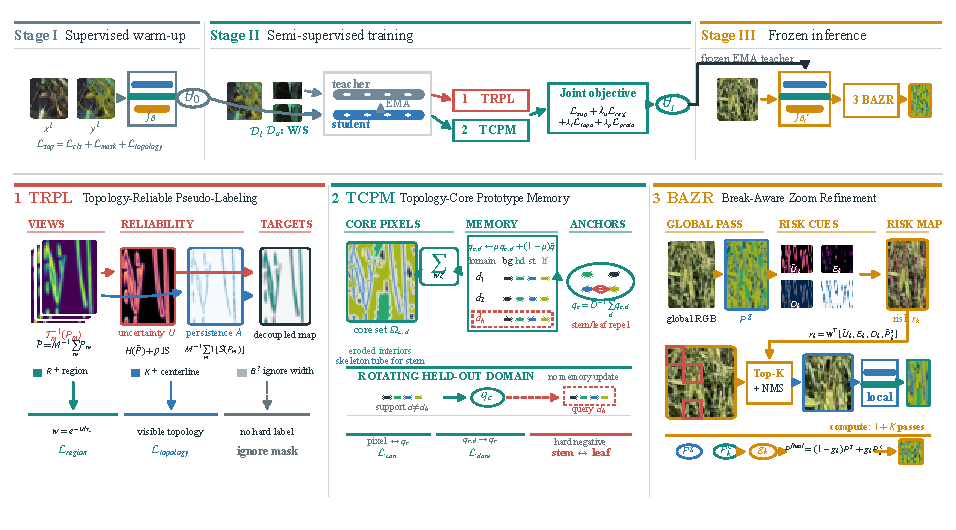
\includegraphics[width=\textwidth]{figures/framework.pdf}
\caption{\METHOD 的三阶段流程与关键算子。上排依次给出监督预热、连续 EMA 教师--学生联合训练和冻结教师推理。下排展开三个创新点：\TRPL 以语义置信度 $Q$ 和双视图分歧 $D$ 形成可靠性 $r$，并用严格骨架共识解耦可靠区域 $R^+$、稳定中心线 $K^+$ 与忽略边界 $B^{?}$；\TCPM 从器官核心 $\Omega_{i,c}$ 分别更新有标注与伪标注类别--域记忆，按样本排除自身采集域后形成类别锚点 $\bar q_c^{(-d_i)}$，再校正可靠区域中偏离该锚点的困难查询；\BAZR 将熵、异常端点、尺度分歧和茎秆先验组合为窗口风险 $r_k$，经 Top-$K$/NMS、局部前向和门控融合得到最终预测。RGB、标注、窗口与裁剪均来自严格对齐的真实样本；底排的概率、可靠性及风险热图依据同一标注几何确定性构造，仅解释空间对齐与运算关系，不表示实验预测。}
\label{fig:framework}
\end{figure}

监督预热、拓扑感知半监督学习与断裂感知推理构成一条连续的信息链（\cref{fig:framework}）。有标注样本首先确定器官语义和茎秆拓扑的共同表征起点 $\theta_0$，教师与学生均由该权重初始化；进入半监督阶段后，教师从第一步起连续执行 EMA，而不再经历冻结后由学生硬覆盖的参数跳变。\TRPL 随后利用无标注图像扩展外观覆盖，将区域可信度与中心线稳定性解耦；\TCPM 把结构可靠核心压缩为跨域类别参照，并将监督传递给同类可靠区域中的困难位置。两条支路共享同一学生特征并通过联合目标相互约束，训练收敛后仅保留 EMA 教师参数 $\theta_t^*$。部署时不再维护学生和原型记忆；\BAZR 从该教师的一次全局前向中评估结构失效风险，把额外计算集中到少量候选窗口。

\subsection{拓扑可靠伪标签学习}
\label{sec:trpl}

\TRPL 借鉴弱到强一致性学习利用教师预测监督强扰动视图的基本形式 \citep{yang2023unimatch}，也保留了 U2PL 和 ST++ 所强调的伪标签可靠性控制 \citep{wang2022u2pl,yang2022stpp}。这些方法把可靠性定义在像素、区域或整幅图像层面，置信度不足的茎秆像素通常被统一丢弃。对小麦图像而言，低置信度并不总意味着器官位置错误：由混合像素和下采样引起的不确定性往往集中在茎秆两侧，而中心位置在不同视图中仍然稳定。soft-clDice 提供了可微的中心线一致性约束 \citep{shit2021cldice}，但它假设监督掩码本身具有可信拓扑，直接用于噪声伪标签可能把偶然误连固化下来。\TRPL 的改动在于先通过多视图一致性确定可见中心线是否可信，再分别处理中心线、区域和边界，而不是对整张伪掩码使用同一阈值或同一拓扑约束。

\subsubsection{双视图可靠性估计}

多组类别阈值与不确定性温度会使伪标签机制难以归因。本文只对无标注图像 $x^u$ 构造原尺度和缩放尺度两个弱视图。第 $m$ 个视图经尺度变换后，其对齐到原图坐标的教师预测为
\begin{equation}
P_m=\mathcal T_m^{-1}
\left(f_{\theta_t}(\mathcal T_m(x^u))\right).
\end{equation}
平均预测 $\bar P=M^{-1}\sum_{m=1}^{M}P_m$ 用于生成类别伪标签 $\hat y(p)=\arg\max_c\bar P_c(p)$。视图分歧采用无需额外温度或权重的总变差距离：
\begin{equation}
D(p)=\frac{1}{2M}\sum_{m=1}^{M}
\left\|P_m(p)-\bar P(p)\right\|_1.
\label{eq:uncertainty}
\end{equation}
将平均预测的最大类别概率记为 $Q(p)=\max_c\bar P_c(p)$，连续可靠性定义为
\begin{equation}
r(p)=Q(p)\left(1-D(p)\right).
\label{eq:confidence}
\end{equation}
$Q$ 衡量语义置信度，$1-D$ 衡量尺度一致性，二者乘积仍位于 $[0,1]$。可靠区域只由一个全局阈值确定，即 $R^+=\{p\mid r(p)\geq\tau_r\}$。

\subsubsection{中心线--区域解耦}

仅使用 $R^+$ 仍容易在边界不确定时删除整个细小茎秆组件。为此，本文先对每个视图的硬茎秆预测执行骨架化：
\begin{equation}
K_m=\mathcal S\!\left(\mathbb I[\arg\max_cP_{m,c}=c_{\mathrm{stem}}]\right),
\end{equation}
再把中心线放回平均预测的茎秆骨架，并要求其在两个视图的一像素邻域内同时出现：
\begin{equation}
K^+=\mathcal S\!\left(\mathbb I[\hat y=c_{\mathrm{stem}}]\right)
\cap\bigcap_{m=1}^{M}\operatorname{Dilate}_1(K_m).
\end{equation}
预测为茎秆但未进入 $R^+$、且邻近可靠茎秆或 $K^+$ 的像素构成不确定边界 $B^{?}$。所有不可靠像素均不进入语义一致性损失，而 $K^+$ 可以绕过区域阈值单独提供正拓扑证据。该表示保留了边界宽度不确定但中心位置稳定的茎秆监督。

\begin{figure}[!htbp]
\centering
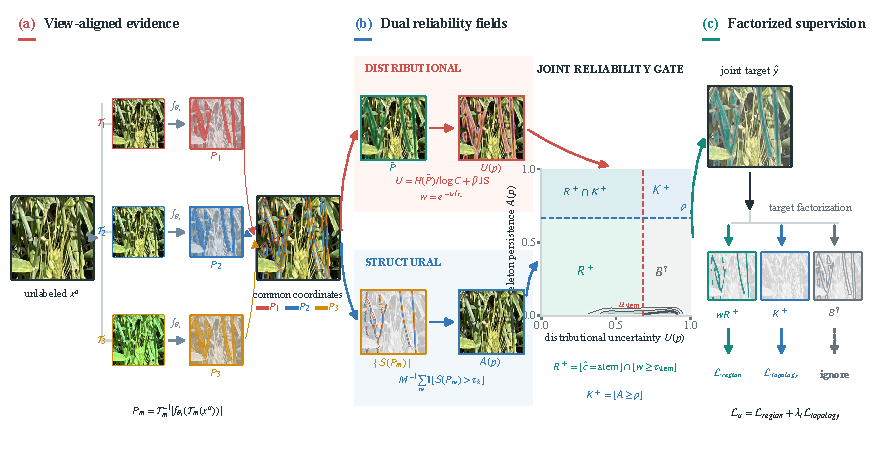
\includegraphics[width=\linewidth]{figures/topology_pseudo_label.pdf}
\caption{\TRPL 的双证据解耦机制。（a）同一幅未标注图像经两个尺度的弱视图和 EMA 教师预测后反变换至公共坐标，形成对齐概率栈 $\{P_m\}$；叠加轮廓揭示了不同视图对茎秆边界宽度的分歧及其共享的轴向结构。（b）分布支路由平均置信度和总变差分歧计算可靠性 $r(p)$，结构支路对齐两个视图的硬预测骨架。单一阈值产生可靠区域，严格骨架交集产生稳定中心线。（c）联合门控在同一空间坐标中分解出加权区域 $rR^+$、稳定中心线 $K^+$ 和忽略边界 $B^{?}$，三者分别连接语义一致性、拓扑一致性和无梯度路径。RGB 来自真实样本；概率场依据其标注几何构造为机制示意，不参与定量结论。}
\label{fig:trpl}
\end{figure}

概率可靠性与结构稳定性的分工在\cref{fig:trpl}中得到直观呈现。记 $\Omega_c=\{p\in R^+\mid\hat y(p)=c\}$，$\mathcal C^+$ 为当前批次中 $\Omega_c$ 非空的类别集合。学生的语义一致性损失采用按类别平均的软 KL：
\begin{equation}
\mathcal L_{\mathrm{semantic}}=
\frac{1}{|\mathcal C^+|}\sum_{c\in\mathcal C^+}
\frac{1}{|\Omega_c|}\sum_{p\in\Omega_c}r(p)
\operatorname{KL}\!\left(\bar P(p)\,\|\,P_s(p)\right),
\label{eq:regionloss}
\end{equation}
其中 $P_s$ 为学生强扰动视图的预测。按类别平均避免背景像素数量支配梯度，软目标则保留教师的类别间不确定性。拓扑监督仅作用于双视图一致的可见中心线：
\begin{equation}
\mathcal L_{\mathrm{topology}}
=-\frac{1}{|K^+|}\sum_{p\in K^+}
\log\max_{q\in\mathcal N_1(p)}P_s^{\mathrm{stem}}(q),
\label{eq:topoloss}
\end{equation}
其中一像素邻域 $\mathcal N_1$ 容忍缩放与反变换造成的离散偏移。最终 $\mathcal L_{\mathrm{TRPL}}=\mathcal L_{\mathrm{semantic}}+\lambda_t\mathcal L_{\mathrm{topology}}$。该设计不对两个可见端点之间执行形态学连线，也不在有标注分支额外叠加损失，因此不会把偶然误连固化或改变监督基线目标。

\subsection{拓扑核心原型记忆}
\label{sec:tcpm}

类别原型为跨域分割提供了紧凑的语义参照。ProDA 根据像素到类别原型的距离修正伪标签并压紧目标域特征 \citep{zhang2021proda}，Pin the Memory 则通过类别记忆和模拟元测试学习未知域中的共享概念 \citep{kim2022pinmemory}。两者启发了本文的原型约束和留一域训练，但直接从完整高置信区域求均值仍不适合小麦器官：叶片边缘、茎秆边缘和二者交叠位置恰好是域风格与分类噪声最强的区域，少量错误像素就可能显著移动像素占比很低的茎秆原型。反过来，若干净核心既用于建库又作为唯一查询，分割头中已经分离的类别质心很容易满足原型分类，损失会退化为近零的自一致性，真正发生域偏移的器官边缘和遮挡邻域反而得不到校正。\TCPM 因而采用非对称证据流：拓扑核心只负责建立稳定锚点，可靠区域中偏离跨域锚点最明显的特征负责接收梯度。

具体地，本文从像素解码器的高分辨率掩码特征中提取归一化表示 $z(p)$，并为样本 $i$ 的类别 $c$ 定义核心像素集合 $\Omega_{i,c}$。茎秆核心由稳定中心线 $K^+$ 及其窄邻域组成；其余类别使用边界收缩后的高置信内部区域。大面积器官可以舍弃少量边界来换取纯净内部特征，茎秆却必须保住窄结构的轴向证据，因此这里不对四个类别使用相同的形态操作。记证据权重 $w(p)$ 在有标注分支取 1、在伪标注分支取 \TRPL 可靠性 $r(p)$。核心在特征分辨率下少于 $n_{\min}$ 个像素时不更新记忆；其余核心先被压缩为带权样本质心
\begin{equation}
\widetilde q_{i,c}=\mathcal N\!\left(
\frac{\sum_{p\in\Omega_{i,c}}w(p)z(p)}
{\sum_{p\in\Omega_{i,c}}w(p)}\right),
\label{eq:corecentroid}
\end{equation}
其中 $\mathcal N(\cdot)$ 表示 $\ell_2$ 归一化。样本质心只用于更新记忆，因而大面积背景不能凭像素数量支配锚点，可靠区域中的混合特征也不会反向污染原型。

有标注核心和伪标注核心分别写入 $q^L_{c,d}$ 与 $q^P_{c,d}$ 两组类别--域记忆：
\begin{equation}
q^s_{c,d}\leftarrow\mathcal N\!\left(
\mu_s q^s_{c,d}+(1-\mu_s)\,
\operatorname{mean}_{i:d_i=d}\widetilde q_{i,c}\right),
\quad s\in\{L,P\}.
\label{eq:domainprototype}
\end{equation}
两组证据不直接混写。伪标注分支仅接收 $w(p)\geq\tau_{\mathrm{mem}}$ 且核心大小不小于 $n_{\min}$ 的样本，并采用更大的 $\mu_P$ 抑制单批伪标签的扰动。对于来自域 $d_i$ 的当前质心，类别参照由其余源域构成：
\begin{equation}
q_c^{s,(-d_i)}=\mathcal N\!\left(
\frac{\sum_{d\neq d_i}a^s_{c,d}q^s_{c,d}}
{\sum_{d\neq d_i}a^s_{c,d}}\right),\qquad
\bar q_c^{(-d_i)}=\mathcal N\!\left(
(1-\eta_t)q_c^{L,(-d_i)}+\eta_t q_c^{P,(-d_i)}\right),
\label{eq:lodoanchor}
\end{equation}
其中 $a^s_{c,d}$ 表示对应记忆是否已经初始化，$0\leq\eta_t\leq\eta_{\max}$。当伪标注参照尚不存在时只使用有标注参照；若不存在可用的有标注参照，则跳过该类别的当前原型项，不让伪标注单独定义语义锚点。该构造对批内每个样本分别排除自身域，而不是在一段迭代中冻结某个固定域；所有满足条件的域仍持续更新，因而不会因为阶段性域冻结形成陈旧原型。

锚点建立后，监督分支以全部有效标注区域作为查询候选，伪标注分支则使用通过 \TRPL 可靠性检验且 $w(p)\geq\tau_q$ 的区域。记样本 $i$、类别 $c$ 的候选集合为 $\mathcal R_{i,c}$，其跨域困难度为
\begin{equation}
h_{i,c}(p)=1-\operatorname{sim}\left(z_i(p),\bar q_c^{(-d_i)}\right),\qquad
\mathcal H_{i,c}=\operatorname{Top}_{\kappa}\{h_{i,c}(p):p\in\mathcal R_{i,c}\},
\label{eq:hardquery}
\end{equation}
其中 $\operatorname{Top}_{\kappa}$ 保留困难度最高的 $\kappa$ 比例。候选过多时先作空间均匀抽样再排序，避免相邻的大面积背景重复占据查询预算。核心像素仍可能进入候选集，但只有偏离留一域锚点的部分会被选中，因此记忆写入和损失读取不再是同一条容易路径。

令 $\mathcal A$ 表示具有正确类别锚点的样本--类别记录集合，$Z_{i,c}=\sum_{p\in\mathcal H_{i,c}}w(p)$。为防止背景等大面积类别支配优化，实现中先在每条样本--类别记录内按置信度归一，再对有效记录等权平均。记 $\mathcal A_{\mathrm{con}}\subseteq\mathcal A$ 为至少存在两个可用类别锚点的记录，$\mathcal C_i^{(-d_i)}$ 为其可用锚点类别集合，则困难查询的原型对比损失为
\begin{equation}
\mathcal L_{\mathrm{con}}=
-\frac{1}{|\mathcal A_{\mathrm{con}}|}
\sum_{(i,c)\in\mathcal A_{\mathrm{con}}}\frac{1}{Z_{i,c}}
\sum_{p\in\mathcal H_{i,c}}w(p)
\log\frac{\exp(\operatorname{sim}(z_i(p),\bar q_c^{(-d_i)})/\tau_p)}
{\sum_{c'\in\mathcal C_i^{(-d_i)}}\exp(\operatorname{sim}(z_i(p),\bar q_{c'}^{(-d_i)})/\tau_p)},
\label{eq:contrastive}
\end{equation}
同类对齐不要求所有域内特征坍缩到同一点，而只惩罚超过容差 $\delta$ 的偏差：
\begin{equation}
\mathcal L_{\mathrm{dom}}=
\frac{1}{|\mathcal A|}\sum_{(i,c)\in\mathcal A}\frac{1}{Z_{i,c}}
\sum_{p\in\mathcal H_{i,c}}w(p)
\left[1-\operatorname{sim}(z_i(p),\bar q_c^{(-d_i)})-\delta\right]_+.
\label{eq:domaincompact}
\end{equation}
对于容易混淆的茎秆与叶片，另设困难负样本项
\begin{equation}
\mathcal L_{\mathrm{hn}}=
\frac{1}{|\mathcal A_{sl}|}\sum_{(i,c)\in\mathcal A_{sl}}\frac{1}{Z_{i,c}}
\sum_{p\in\mathcal H_{i,c}}w(p)
\left[m+\operatorname{sim}(z_i(p),\bar q_{c^-}^{(-d_i)})
-\operatorname{sim}(z_i(p),\bar q_c^{(-d_i)})\right]_+,
\label{eq:hardnegative}
\end{equation}
其中 $\mathcal A_{sl}\subseteq\mathcal A$ 只包含叶片和茎秆锚点均可用的对应记录，$c^-$ 是二者中的另一类别；任一有效集合为空时相应损失记为 0。三项均采用固定查询上限、逐记录类平衡和置信加权，只有困难区域产生原型梯度；核心锚点、容易区域以及容差内的合理域内变化不会被反复压缩。

TCPM 并不随半监督阶段立即全量启用。监督最优权重同步到师生两支后，以 Stage II 的第 0 次迭代为 $t_0$：$[t_0,t_1)$ 只积累有标注记忆，不施加原型损失；$[t_1,t_2)$ 将三项损失由 0 线性增加到设定权重；到 $t_2$ 后才允许满足质量门限的伪标注核心更新第二组记忆，并在随后若干迭代内把 $\eta_t$ 从 0 增至 $\eta_{\max}$。该日程把“教师是否连续更新”和“原型何时参与优化”分开管理，避免中途教师替换与原型启用在同一节点叠加。

\begin{figure}[!htbp]
\centering
%\includegraphics[width=\linewidth]{figures/topology_core_memory.pdf}
\fbox{\parbox{0.94\linewidth}{\centering \vspace{1.05cm}
\placeholder{TCPM 机理图采用“干净核心写入--双记忆聚合--留一域锚点--困难可靠查询”四段式横向流程，并在底部增加独立课程时间轴。第一段在同一幅小麦 RGB、类别掩码和特征网格上同时画两类区域：茎秆核心使用红色骨架窄管，麦穗、叶片和背景核心使用向内收缩的深色实心区域；核心外但通过可靠性检验的器官区域使用浅色半透明覆盖，灰色斜线表示忽略边界。深色核心经置信加权汇聚为样本--类别质心 $\widetilde q_{i,c}$，少于 4 个特征像素时以虚线箭头指向“skip”；浅色区域不得连接记忆写入口。第二段上下排列有标注记忆 $q^L_{c,d}$ 与伪标注记忆 $q^P_{c,d}$，横轴为背景、麦穗、茎秆和叶片，纵轴为 Domain 1 至 Domain 9；实线 EMA 箭头标注 $\mu_L=0.95$，较细虚线箭头标注 $\mu_P=0.995$，伪核心写入口前画 $w\geq0.8$ 门控，两组记忆之间不画直接写入箭头。第三段以灰色横条遮掉当前样本的第 $d_i$ 行，其余域分别聚合为 $q_c^{L,(-d_i)}$ 和 $q_c^{P,(-d_i)}$，再用标有 $(1-\eta_t)$ 与 $\eta_t$ 的两条不同粗细箭头融合为 $\bar q_c^{(-d_i)}$；用两个来自不同当前域的小例子强调排除操作逐样本改变，而所有域仍继续写入。第四段从浅色可靠区域中先做最多 128 点的空间均匀采样，伪标注查询入口标注 $w\geq0.6$，每个点以细线连接正确类别锚点；按余弦距离着色，从蓝色易查询过渡到红色困难查询，仅用粗描边保留距离最高的 25\%。红色查询分别连接原型分类损失、带容差 $\delta$ 的同类对齐损失和叶片--茎秆排序损失；蓝色易查询和容差圆内部画断开的灰色梯度符号，明确其不产生重复压缩。右侧配一组共享坐标轴的前后散点图，展示困难边缘特征向正确锚点移动，而深色核心锚点和合理类内散布基本保持。底部时间轴以 Stage II 为零点，依次标出 0--5k“仅写 $q^L$”、5--15k“损失线性升权”、15k“开放高质量 $q^P$”、25k“$\eta_t=0.2$”；时间轴上方另画教师与学生从同一监督 checkpoint 出发、EMA 连续更新的两条轨迹，禁止出现 20k 硬复制箭头。测试目标域以独立虚线灰框放在全部记忆之外。类别、域、标注来源、写入/读取和有/无梯度箭头必须使用互不混淆且不遮挡组件的图例。}
\vspace{1.05cm}}}
\caption{\TCPM 以拓扑核心建立课程式双记忆，并用逐样本留一域锚点校正可靠区域中的困难查询。}
\label{fig:tcpm}
\end{figure}

如\cref{fig:tcpm}所示，双记忆把人工标注的稳定参照与伪标注带来的外观覆盖分开管理，逐样本留一域只改变当前损失所读取的参照，不阻断任何源域的正常写入。核心--查询非对称性进一步把“哪些特征可信”与“哪些特征需要校正”分开：前者决定锚点，后者决定梯度位置，从而避免容易核心形成近零损失，也避免边缘噪声移动记忆。

\subsection{断裂感知选择性放大}
\label{sec:bazr}

选择性细化并非新的计算范式。PointRend 在不确定点上迭代预测以恢复清晰边界 \citep{kirillov2020pointrend}。Liu 等人的 SparseRefine 用预测熵筛选少量高分辨率像素 \citep{liu2024sparserefine}，HRDA 也说明局部高分辨率与全局上下文需要共同保留 \citep{hoyer2022hrda}。这些方法主要把高熵或边界视为细化依据；对于小麦茎秆，一段预测可以具有较高置信度却在低分辨率下发生断裂，普通叶片边缘又可能具有高熵但并不需要额外计算。项目原方案采用密集多尺度滑窗缓解这一问题 \citep{cao2025detailminority}，代价是所有位置都被重复处理。\BAZR 沿用“把高分辨率计算留给困难位置”的思想，但把路由单位从像素改为窗口，并把结构断裂而非单纯分类不确定性纳入选择标准。

\BAZR 对完整图像执行一次全局推理，得到概率图 $P^g$。为避免在路由阶段再次运行完整多尺度模型，本文在像素解码器的高、低分辨率特征上设置轻量辅助预测头，并在同一次前向过程中得到 $P^{\mathrm{high}}_{\mathrm{aux}}$ 和 $P^{\mathrm{low}}_{\mathrm{aux}}$。

将图像划分为候选窗口 $\{\mathcal W_k\}$。第 $k$ 个窗口的细化优先级为
\begin{equation}
r_k=
a\,\overline U_k
+b\,E_k
+c\,D_k
+d\,\overline P^{g,\mathrm{stem}}_k,
\label{eq:routingscore}
\end{equation}
其中 $\overline U_k$ 为全局预测的平均归一化熵，$E_k$ 为异常骨架端点密度，$D_k$ 为两个辅助预测头在茎秆类别上的平均差异，$\overline P^{g,\mathrm{stem}}_k$ 为平均茎秆概率。$E_k$ 使模型关注可能发生断裂的细长组件，$D_k$ 则反映网络内部不同空间尺度对该区域的判断分歧。

本文使用非极大值抑制去除高度重叠窗口，并选择得分最高的 $K$ 个窗口。每个窗口从原始图像裁剪后放大至网络输入尺寸，复用同一分割器得到局部高分辨率预测 $P_k^z$。局部与全局预测通过轻量门控函数融合：
\begin{equation}
P^{\mathrm{final}}(p)=
g_k(p)P_k^z(p)
+[1-g_k(p)]P^g(p),
\quad p\in\mathcal W_k,
\label{eq:fusion}
\end{equation}
窗口外保持 $P^{\mathrm{final}}=P^g$。门控函数在有标注源域和高可靠伪标签上训练，不使用目标域标签。最终推理仅需 $1+K$ 次分割器前向计算。

\begin{figure*}[!htbp]
\centering
%\includegraphics[width=\linewidth]{figures/selective_zoom.pdf}
\fbox{\parbox{0.94\linewidth}{\centering \vspace{1.0cm}
\placeholder{BAZR 机理图以一张包含细茎、叶片交叠和大面积背景的小麦图像为起点。顶部为单次全局前向，主预测头、高分辨率辅助头和低分辨率辅助头从共享特征同时输出结果。中部四张与原图对齐的热图依次表示归一化熵 $U$、异常骨架端点密度 $E$、两个辅助头的茎秆分歧 $D$ 和全局茎秆概率；相同候选网格覆盖四张热图，四项信号按照 $a$、$b$、$c$、$d$ 加权形成窗口分数 $r_k$。NMS 模块滤除重叠候选并保留带编号的 Top-$K$ 窗口，各窗口从原始分辨率 RGB 中裁剪、放大并送入共享分割器，局部结果经空间门控 $g_k$ 与全局预测融合。右侧局部对照标记了断裂茎秆的连接恢复以及保持不变的正确叶片边界。底部比较两条计算路径：密集多尺度方案以覆盖全图的滑窗产生约 160 次前向，BAZR 由一次全局前向和 $K$ 次局部前向组成；反事实案例分别显示未被选择的高熵普通叶片边界，以及被选中的中等熵异常断茎。}
\vspace{1.0cm}}}
\caption{\BAZR 根据茎秆结构失效风险分配高分辨率计算，而非均匀处理整幅图像。}
\label{fig:bazr}
\end{figure*}

熵与结构风险对计算路由的不同作用在\cref{fig:bazr}中得到对照。只有当窗口得分得到多源证据共同支持时，局部预测才会替换全局结果；门控融合则限制修正范围，避免高分辨率裁剪失去全局上下文后破坏已经正确的区域。

\subsection{训练目标与优化过程}

有标注数据仅使用 Mask2Former 原有的类别、掩码交叉熵和 Dice 损失，记为 $\mathcal L_{\mathrm{sup}}$；这保证监督分支与统一主干基线完全一致。原型学习损失为
\begin{equation}
\mathcal L_{\mathrm{prototype}}
=\mathcal L_{\mathrm{con}}
+\gamma\mathcal L_{\mathrm{dom}}
+\xi\mathcal L_{\mathrm{hn}}.
\end{equation}
局部融合门控的监督记为 $\mathcal L_{\mathrm{route}}$。完整训练目标为
\begin{equation}
\mathcal L=
\mathcal L_{\mathrm{sup}}
+\lambda_u\mathcal L_{\mathrm{TRPL}}
+\lambda_p\mathcal L_{\mathrm{prototype}}
+\lambda_r\mathcal L_{\mathrm{route}}.
\label{eq:total}
\end{equation}

训练由监督预热和半监督联合优化组成。监督预热只使用有标注图像，模型选择后将同一组最优参数同时加载到教师和学生；二者不存在重新初始化的分割头。进入联合优化后，学生同时接收有标注图像与按域均衡采样的无标注图像，教师从第一步起按\cref{eq:ema}连续更新。TCPM 同步清空记忆，但前 5,000 次只写入有标注核心，随后逐步开放困难查询损失和高质量伪标注记忆；逐样本留一域参照随当前样本动态构造，不设置固定域冻结周期。具体权重与训练节点见\cref{sec:implementation}。


\section{实验}
\label{sec:experiments}

\subsection{数据集与评测协议}
\label{sec:datasets}

\paragraph{少标注跨域协议}
GWFSS 竞赛发布的少标注协议包含来自 9 个源域的 99 张像素级标注训练图像、64,368 张无标注训练图像和 99 张验证图像，另有来自未见域的 110 张测试图像；所有图像均被裁剪为 $512\times512$ 像素。该协议同时考查无标注数据利用和未知采集域泛化。模型选择、超参数调整和消融实验仅依据源域验证集完成，测试集仅用于最终评测，以避免目标域信息泄漏。除非另有说明，所有对比方法均使用相同的 99 张标注图像。

\paragraph{完整数据区域协议}
数据集论文给出的地域划分进一步检验了模型对特定少标注拆分的依赖程度。完整数据包含 1,096 张精细标注图像和 52,078 张无标注图像，覆盖 11 个研究机构、不同成像平台和约 $0.09$--$0.71$ mm/pixel 的地面采样距离 \citep{wang2025gwfss}。训练域来自 Arvalis、CIMMYT、ETHZ、INRAE、NJAU、RRES 和 ULiege，UTokyo 作为验证域，UQ 作为测试域。实验保持官方地域划分不变，并分别使用训练域中 10\%、25\%、50\% 和 100\% 的标注图像；各比例由固定随机种子分层采样，且在所有方法之间共享。不同采集条件下的局部标注细节见\cref{fig:dataset}，基于全部标注图像的域级统计与器官尺度负担分别见\cref{fig:domain-fingerprint,fig:organ-scale-burden}。

\begin{figure}[!htbp]
\centering
%\includegraphics[width=\linewidth]{figures/dataset_domains.pdf}
\fbox{\parbox{0.94\linewidth}{\centering \vspace{1.05cm}
\placeholder{数据域图版由四列三行构成，四列分别对应近距离高分辨率、远距离低分辨率、强阴影绿色冠层和衰老黄色冠层。第一行给出原始 RGB，第二行叠加背景、麦穗、茎秆和叶片的固定颜色标注，第三行显示相同位置的局部放大。列标题标记机构或域编号，底部短标签列出地面采样距离、生育阶段、视角和主要干扰。两个放大框分别定位叶茎交叠处的类别歧义，以及低分辨率下仅有 1--3 像素宽的茎秆。训练域采用实线边框，未知测试域采用虚线边框，图例注明该域在训练中不可见。}
\vspace{1.05cm}}}
\caption{GWFSS 不同采集域的图像、像素级标注与局部细节。实线框和虚线框分别表示源域与未知测试域，局部放大区域呈现了叶茎交叠和低分辨率细茎两类主要困难。}
\label{fig:dataset}
\end{figure}

\begin{figure*}[!htbp]
\centering
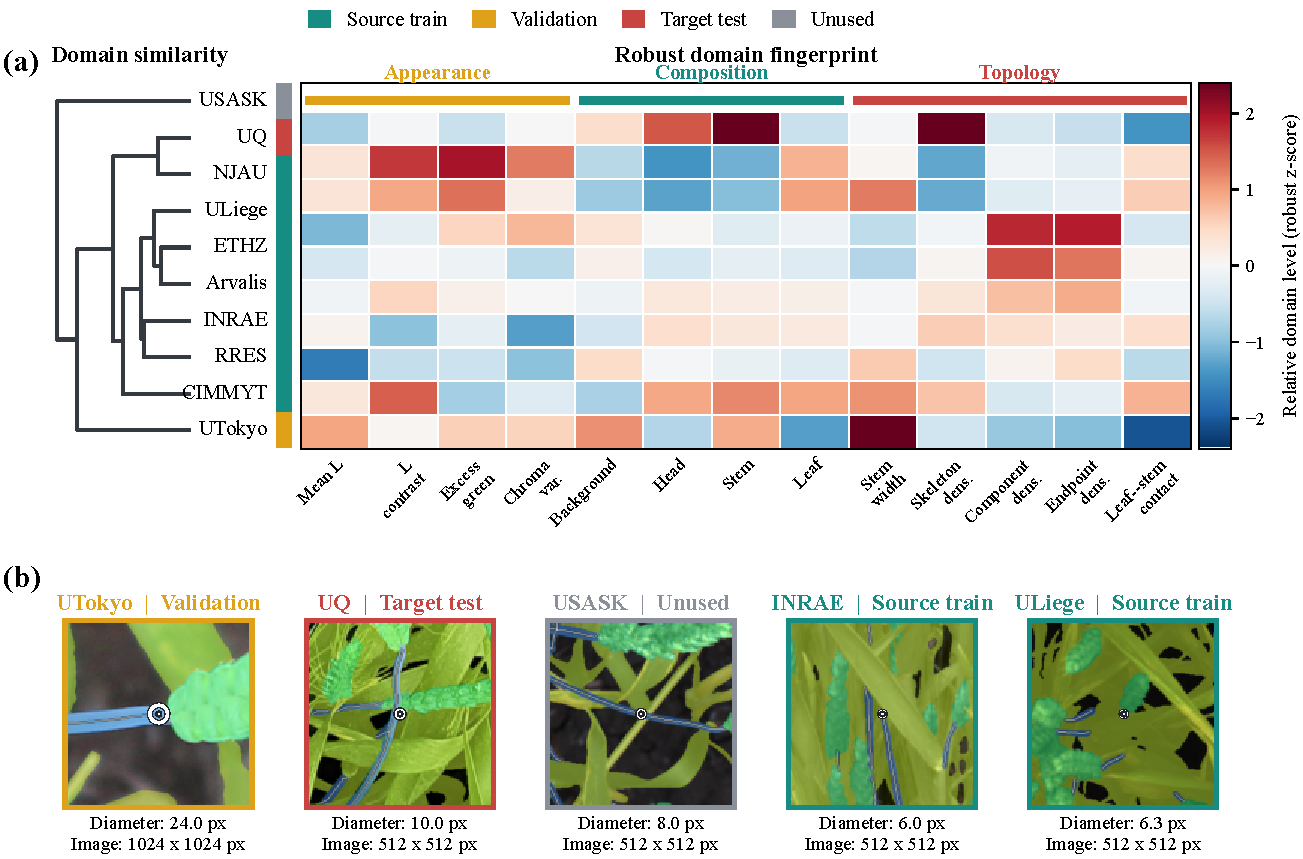
\includegraphics[width=\textwidth]{figures/domain_morphology_fingerprint.pdf}
\caption{完整标注子集的跨域外观、器官组成与拓扑形态指纹。(a) 对每个域的 13 项图像与标注统计取中位数，并以跨域中位数和四分位距标准化；树状图采用标准化指纹的欧氏距离和平均连接法。侧边色带表示该域在地域协议中的作用。(b) 在具有有效茎秆骨架的图像中，自动选取最接近各域中位指纹的样本，并以相同的 $256\times256$ 原生像素视野显示局部区域。白线表示茎秆中轴，圆环表示中位宽度测量点处的最大内切圆。绿色、蓝色和黄绿色叠加区域分别为麦穗、茎秆和叶片标注。}
\label{fig:domain-fingerprint}
\end{figure*}

用于上述统计的 1,096 张图像在标注子集中对应 10 个具有类别掩码的采集域。由\cref{fig:domain-fingerprint}可见，验证域 UTokyo 和目标测试域 UQ 到七个源域中心的标准化距离分别为 6.32 和 3.97，均超过任一单独源域到该中心的最大距离 3.27。UQ 的主要偏移同时出现在绿色过量指数（$+1.95$）、色度变化（$+1.58$）、亮度对比度（$+1.55$）和麦穗面积占比（$-1.41$）上，括号内为相对源域中心的稳健标准化差值。

图中的茎宽描述标注栅格上的局部直径，而非小麦茎秆的物理直径。对二值茎秆掩码进行骨架化后，以 $D(p)$ 表示骨架像素 $p$ 到最近背景像素的欧氏距离，单幅图像的茎宽定义为 $\operatorname{median}_{p\in S}2D(p)$，域级数值再取域内图像的中位数。UTokyo 标注图像为 $1024\times1024$，其余九个标注域为 $512\times512$；因此 UTokyo 的域中位宽度 22.8 px 与 UQ 代表样本的 10.0 px 不能直接解释为前者具有更粗的物理茎秆。该统计反映的是模型所需处理的原生栅格尺度变化，\cref{fig:domain-fingerprint}(b) 也据此采用固定原生像素大小的裁块，而不再把不同分辨率的整幅图像缩放到相同显示尺寸。结合器官面积占比和叶--茎接触统计可知，地域迁移同时改变了成像外观、器官组成和细长结构的像素表达，单纯的颜色增强无法覆盖后两类变化；本文因而在伪标签可靠性和跨域原型构建中显式保留器官拓扑信息。

\begin{figure*}[!htbp]
\centering
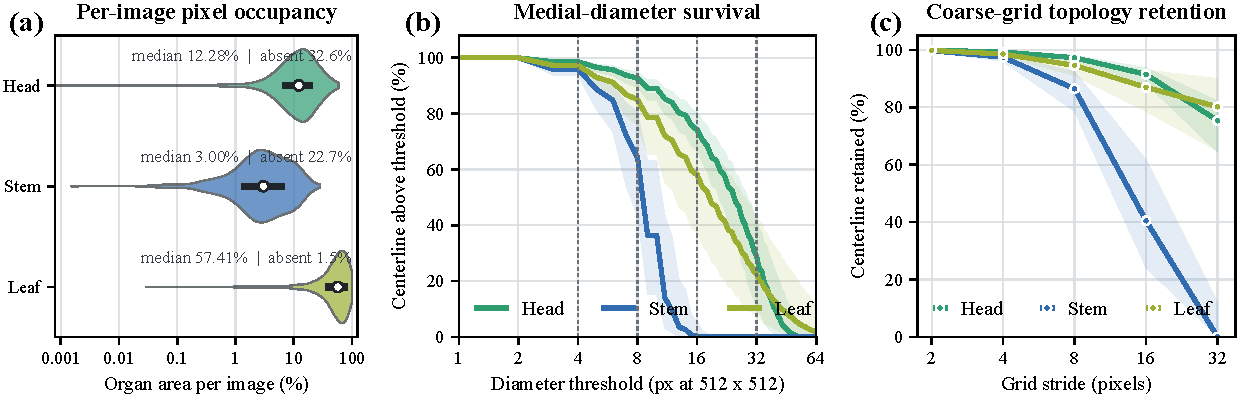
\includegraphics[width=\textwidth]{figures/organ_scale_burden.pdf}
\caption{统一尺度下的器官像素负担与几何生存性。(a) 每幅图像中非零器官面积占比的对数分布，白点和黑线分别表示中位数与四分位区间，文字同时给出器官缺失图像的比例。(b) 骨架局部直径生存曲线，即局部直径不小于给定阈值的中心线比例；实线和阴影分别为跨图像中位数与四分位区间，虚线标出常见特征步长。(c) 以网格内器官占比不低于 50\% 为保留条件，将真值投影到不同步长的粗网格后，原始中心线仍被覆盖的比例。所有掩码均以最近邻插值统一为 $512\times512$；粗网格投影仅用于几何诊断，不代表网络预测。}
\label{fig:organ-scale-burden}
\end{figure*}

器官占比和结构宽度呈现出一致的茎秆劣势，相关分布汇总于\cref{fig:organ-scale-burden}(a)。在器官实际出现的图像中，茎秆面积中位数仅为 3.00\%，麦穗和叶片则分别为 12.28\% 和 57.41\%。麦穗在 32.6\% 的图像中缺失，反映了数据覆盖多个生育期；即使排除器官缺失造成的零值，茎秆的像素监督仍明显少于另外两类器官。

将全部掩码统一到 $512\times512$ 后，茎秆、叶片和麦穗的图像级中位局部直径依次为 8.25、18.11 和 24.17 px。茎秆中心线中有 35.7\% 的局部直径不足 8 px，而叶片和麦穗的对应比例仅为 15.0\% 和 7.3\%。这种尺度差异在粗网格诊断中产生非线性后果：stride 8 时三类器官的中位中心线保留率分别为 86.4\%、94.6\% 和 97.2\%，stride 16 时茎秆骤降至 40.5\%，叶片和麦穗仍保持 87.0\% 和 91.5\%。多数栅格化没有模拟卷积特征的学习能力，但它排除了纹理和类别置信度的影响，单独揭示了离散采样对细长结构施加的几何压力。这一结果解释了为何茎秆监督需要保留稳定中心线，也说明局部放大应优先分配给发生结构断裂的区域，而不是均匀增加所有器官的推理分辨率。

\subsection{评价指标}

遵循数据集论文，本文以四类平均交并比（mIoU）作为主要指标，并同时报告背景、麦穗、茎秆和叶片的类别 IoU。类别 $c$ 的 IoU 定义为
\begin{equation}
\operatorname{IoU}_c=
\frac{\operatorname{TP}_c}
{\operatorname{TP}_c+\operatorname{FP}_c+\operatorname{FN}_c},
\qquad
\operatorname{mIoU}=\frac{1}{C}\sum_{c=1}^{C}\operatorname{IoU}_c .
\end{equation}
整体 mIoU 容易掩盖像素占比较低类别的变化，因此实验将茎秆 IoU 作为核心辅助指标。二值茎秆掩码上的 soft-clDice \citep{shit2021cldice}、骨架精确率、骨架召回率和边界 F-score 则分别度量中心线重合、结构检出和轮廓质量。所有结构指标采用相同的骨架化参数和边界容差。

效率评测报告参数量、FLOPs、单张图像延迟、峰值显存和分割器前向次数。延迟包含裁剪、窗口选择和局部结果融合，并在相同硬件、批大小及预热设置下测量。密集多尺度滑窗方法的前向次数按实际裁剪数统计，\BAZR 的对应计算量为 $1+K$ 次前向。

\subsection{实现细节}
\label{sec:implementation}

基础网络由 BEiTv2-Large、ViT-Adapter、Mask2Former 和 SAPA 构成 \citep{peng2022beitv2,chen2023vitadapter,cheng2022mask2former,lu2022sapa}。编码器采用 ImageNet-1K 预训练权重，输入裁剪尺寸为 $512\times512$。AdamW 优化器的解码器初始学习率为 $1\times10^{-4}$，编码器学习率乘子为 0.1，权重衰减为 0.05。监督预热和半监督联合训练分别执行 20,000 和 90,000 次迭代；联合训练的全局批大小为 2 张有标注图像和 2 张无标注图像。弱增强包括多尺度短边缩放、$512\times512$ 随机裁剪、SSD 颜色扰动和随机水平翻转，学生分支额外采用颜色抖动、随机灰度和高斯模糊。EMA 动量设为 0.9996，前 20,000 次联合训练迭代作为教师冻结阶段。

\TRPL 使用原尺度与 0.75 倍尺度两个教师视图，背景、麦穗、茎秆和叶片的置信阈值依次为 0.70、0.70、0.55 和 0.70。不确定性权重 $\beta$ 和温度 $\tau_u$ 分别为 1.0 和 0.5，最大可接受不确定性为 0.75；骨架阈值、持续性阈值和边界半径分别为 0.35、0.5 和 2 像素。区域 Dice、拓扑和骨架一致性损失的权重依次为 0.5、0.5 和 0.25。\TCPM 使用 9 组域记忆，原型动量 $\mu$ 为 0.99，对比温度 $\tau_p$ 为 0.1，每类每次最多采样 256 个核心像素，留出域每 1,000 次迭代轮换一次。对比、域紧致和困难负样本损失的权重分别为 0.1、0.05 和 0.05。\BAZR 从步长为 128 的 $256\times256$ 候选窗口中选择 $K=4$ 个区域，将其放大到 $512\times512$，NMS 阈值设为 0.3；熵、异常端点、尺度分歧和茎秆概率的路由权重依次为 1.0、2.0、1.0 和 0.5。

所有主结果采用 3 个固定随机种子报告均值与标准差。训练和推理在 NVIDIA A100 上完成，代码基于 PyTorch 1.9.0、CUDA 11.1 和 Detectron2 0.6 实现。

\subsection{与现有方法的比较}

\paragraph{少标注跨域结果}
Cao 等人的方法结合 Guided Distillation、器官分布筛选和密集多尺度滑窗，在验证集与未知域测试集上分别取得 77.04\% 和 74.68\% mIoU \citep{cao2025detailminority}。DeCon 通过持续预训练、无标注样本选择和不确定性过滤得到 73.61\% 和 67.88\% \citep{ghosh2025decon}。统一主干监督基线、两种已有方法和本文方法的结果汇总于\cref{tab:small-label-main}，其中结构指标与实际前向次数用于区分训练收益和测试时计算收益。

\begin{table*}[!htbp]
\centering
\caption{GWFSS 少标注跨域协议上的定量比较。mIoU、Stem IoU 和 clDice 的单位为百分数，``--'' 表示原论文未报告相应结果，前向次数按每张 $512\times512$ 测试图像统计。}
\label{tab:small-label-main}
\resizebox{\textwidth}{!}{
\begin{tabular}{lccccccc}
\toprule
方法 & 主干网络 & 使用无标注数据 & 验证 mIoU & 测试 mIoU & Stem IoU & Stem clDice & 前向次数 \\
\midrule
监督基线 & BEiTv2-L & 否 & \placeholder{XX.XX} & \placeholder{XX.XX} & \placeholder{XX.XX} & \placeholder{XX.XX} & 1 \\
DeCon \citep{ghosh2025decon} & ConvNeXt-L/BEiT-L & 是 & 73.61 & 67.88 & -- & -- & -- \\
Cao 等 \citep{cao2025detailminority} & BEiTv2-L & 是 & 77.04 & 74.68 & -- & -- & $\sim160$ \\
\METHOD（全局推理） & BEiTv2-L & 是 & \placeholder{XX.XX} & \placeholder{XX.XX} & \placeholder{XX.XX} & \placeholder{XX.XX} & 1 \\
\METHOD（\BAZR） & BEiTv2-L & 是 & \placeholder{XX.XX} & \placeholder{XX.XX} & \placeholder{XX.XX} & \placeholder{XX.XX} & 5 \\
\bottomrule
\end{tabular}}
\end{table*}

监督基线从验证域迁移到未知测试域时下降了 \placeholder{X.XX} 个百分点，而 \METHOD 将该差距缩小到 \placeholder{X.XX} 个百分点，并相对监督基线提高测试 mIoU \placeholder{X.XX} 个百分点。这一变化表明性能增益并非只来自对 99 张标注图像的进一步拟合。对细长结构的改善更为集中：Stem IoU、clDice 和边界 F-score 分别提高 \placeholder{X.XX}、\placeholder{X.XX} 和 \placeholder{X.XX} 个百分点。clDice 的增幅高于边界 F-score，说明主要收益来自茎秆断裂的减少，而非预测区域的均匀膨胀。

全局推理与 \BAZR 共享完全相同的模型权重，两者的测试 mIoU 相差 \placeholder{X.XX} 个百分点，因而该增益可以归因于局部高分辨率细化。默认 $K=4$ 时每幅图像仅执行 5 次分割器前向，相比密集多尺度滑窗约 160 次前向减少了 96.9\% 的调用；实测延迟由 \placeholder{XXXX ms} 降至 \placeholder{XXX ms}。精度和计算量的共同变化说明，结构风险能够比均匀滑窗更有效地分配测试时预算。

\paragraph{完整数据区域泛化结果}
地域划分比随机拆分更直接地暴露采集域偏移。数据集论文中，SegFormer-B1 的 mIoU 为 60.64\%，其中茎秆 IoU 仅为 19.23\%；DeepLabV3+ 的两项结果分别为 52.15\% 和 6.64\% \citep{wang2025gwfss}。同一划分上的统一主干监督基线与 \METHOD 结果也列入\cref{tab:region-main}，从而控制网络容量差异。

\begin{table}[!htbp]
\centering
\caption{完整 GWFSS 数据地域划分上的类别 IoU 与 mIoU（\%）。}
\label{tab:region-main}
\resizebox{\linewidth}{!}{
\begin{tabular}{lccccc}
\toprule
方法 & 背景 & 麦穗 & 茎秆 & 叶片 & mIoU \\
\midrule
DeepLabV3+ \citep{wang2025gwfss} & 74.32 & 46.25 & 6.64 & 81.40 & 52.15 \\
SegFormer-B1 \citep{wang2025gwfss} & 75.46 & 66.11 & 19.23 & 81.75 & 60.64 \\
统一主干监督基线 & \placeholder{XX.XX} & \placeholder{XX.XX} & \placeholder{XX.XX} & \placeholder{XX.XX} & \placeholder{XX.XX} \\
\METHOD & \placeholder{XX.XX} & \placeholder{XX.XX} & \placeholder{XX.XX} & \placeholder{XX.XX} & \placeholder{XX.XX} \\
\bottomrule
\end{tabular}}
\end{table}

在未知地域上，\METHOD 相对统一主干监督基线提高 mIoU \placeholder{X.XX} 个百分点，其中茎秆获得最大的类别增益 \placeholder{X.XX} 个百分点；背景和叶片分别变化 \placeholder{X.XX} 和 \placeholder{X.XX} 个百分点。类别间的不均匀增益与 \TCPM 的采样机制一致。大面积器官从收缩后的内部区域已能得到稳定原型，而像素稀少的茎秆从中心线核心中获益更明显，边界混合像素对其类别中心的牵引随之减弱。源域平均 mIoU 仅变化 \placeholder{X.XX} 个百分点，最差源域和未知域则分别提高 \placeholder{X.XX} 和 \placeholder{X.XX} 个百分点。这组差异进一步表明，原型约束主要改善了跨域稳定性，而非对易分源域提供一般性的容量增益。

\subsection{消融实验}
\label{sec:ablation}

\paragraph{三个模块的增量作用}
模块消融从同一监督基线出发，并保持主干、数据和训练预算不变。训练阶段依次引入 \TRPL 与 \TCPM，\BAZR 只改变推理路径，因此启用 \TCPM 的最后两组共享模型权重。各模块带来的增量结果见\cref{tab:module-ablation}。

\begin{table*}[!htbp]
\centering
\caption{三个模块在少标注协议上的增量消融。$\checkmark$ 表示启用对应模块，所有指标均在相同数据划分下计算。}
\label{tab:module-ablation}
\begin{tabular}{ccccccccc}
\toprule
\TRPL & \TCPM & \BAZR & 验证 mIoU & 测试 mIoU & Stem IoU & Stem clDice & Boundary F & 前向次数 \\
\midrule
 & & & \placeholder{XX.XX} & \placeholder{XX.XX} & \placeholder{XX.XX} & \placeholder{XX.XX} & \placeholder{XX.XX} & 1 \\
$\checkmark$ & & & \placeholder{XX.XX} & \placeholder{XX.XX} & \placeholder{XX.XX} & \placeholder{XX.XX} & \placeholder{XX.XX} & 1 \\
$\checkmark$ & $\checkmark$ & & \placeholder{XX.XX} & \placeholder{XX.XX} & \placeholder{XX.XX} & \placeholder{XX.XX} & \placeholder{XX.XX} & 1 \\
$\checkmark$ & $\checkmark$ & $\checkmark$ & \placeholder{XX.XX} & \placeholder{XX.XX} & \placeholder{XX.XX} & \placeholder{XX.XX} & \placeholder{XX.XX} & 5 \\
\bottomrule
\end{tabular}
\end{table*}

引入 \TRPL 后，Stem IoU 和 clDice 分别提高 \placeholder{X.XX} 和 \placeholder{X.XX} 个百分点，而 mIoU 增幅为 \placeholder{X.XX} 个百分点。结构指标更显著的变化表明，区域平均指标确实弱化了细茎连续性的改善。进一步加入 \TCPM 后，源域验证与未知域测试 mIoU 分别变化 \placeholder{X.XX} 和 \placeholder{X.XX} 个百分点；更大的测试域增益符合域级记忆对未知条件的约束作用。在相同权重上启用 \BAZR 又将 Stem IoU 提高 \placeholder{X.XX} 个百分点。逐图错误分析显示，\TRPL 消除的训练噪声断裂与 \BAZR 修复的推理断裂仅有 \placeholder{XX.X\%} 重合，说明二者处理的是互补误差，而非重复优化同一批样本。

\paragraph{伪标签结构设计}
固定阈值、多视图不确定性和中心线--区域解耦使用相同的教师预测，差别仅在伪标签进入损失的方式。源域验证标签在训练期间保持隐藏，只用于离线计算接纳率和中心线准确率。具体结果汇总于\cref{tab:trpl-ablation}。

\begin{table}[!htbp]
\centering
\caption{伪标签可靠性建模的消融结果。接纳率衡量进入无监督损失的像素比例，中心线准确率在隐藏的验证标注上离线计算。}
\label{tab:trpl-ablation}
\resizebox{\linewidth}{!}{
\begin{tabular}{lcccc}
\toprule
伪标签策略 & 接纳率 & 中心线准确率 & Stem IoU & clDice \\
\midrule
固定类别阈值 & \placeholder{XX.XX} & \placeholder{XX.XX} & \placeholder{XX.XX} & \placeholder{XX.XX} \\
熵不确定性 & \placeholder{XX.XX} & \placeholder{XX.XX} & \placeholder{XX.XX} & \placeholder{XX.XX} \\
多视图不确定性 & \placeholder{XX.XX} & \placeholder{XX.XX} & \placeholder{XX.XX} & \placeholder{XX.XX} \\
中心线--区域解耦（\TRPL） & \placeholder{XX.XX} & \placeholder{XX.XX} & \placeholder{XX.XX} & \placeholder{XX.XX} \\
\bottomrule
\end{tabular}}
\end{table}

单纯采用熵过滤使接纳率由 \placeholder{XX.XX\%} 变为 \placeholder{XX.XX\%}，但中心线准确率只提高 \placeholder{X.XX} 个百分点，表明像素置信度无法充分区分边界模糊与位置错误。多视图分歧进一步排除了跨尺度不稳定区域，中心线准确率提高到 \placeholder{XX.XX\%}。完整 \TRPL 在保持 \placeholder{XX.XX\%} 接纳率的同时，将 Stem IoU 和 clDice 分别提高 \placeholder{X.XX} 和 \placeholder{X.XX} 个百分点，断裂组件数下降 \placeholder{XX.X\%}。接纳率并未与结构指标同步增加，说明收益来自监督证据的重新组织，而非简单扩大伪标签覆盖范围。

\paragraph{原型来源与域泛化}
原型消融逐步改变均值计算所使用的像素集合，并单独移除留一域模拟。除平均性能外，实验还记录最差源域 mIoU，以降低样本量和域难度差异对平均值的掩盖。不同原型证据的比较见\cref{tab:prototype-ablation}。

\begin{table}[!htbp]
\centering
\caption{原型证据来源与留一域训练的消融结果。最差源域 mIoU 为各源域独立评测结果中的最小值。}
\label{tab:prototype-ablation}
\resizebox{\linewidth}{!}{
\begin{tabular}{lccc}
\toprule
原型策略 & 验证 mIoU & 最差源域 mIoU & 测试 mIoU \\
\midrule
无原型 & \placeholder{XX.XX} & \placeholder{XX.XX} & \placeholder{XX.XX} \\
完整高置信区域 & \placeholder{XX.XX} & \placeholder{XX.XX} & \placeholder{XX.XX} \\
收缩内部区域 & \placeholder{XX.XX} & \placeholder{XX.XX} & \placeholder{XX.XX} \\
拓扑核心，无留一域模拟 & \placeholder{XX.XX} & \placeholder{XX.XX} & \placeholder{XX.XX} \\
拓扑核心与留一域模拟（\TCPM） & \placeholder{XX.XX} & \placeholder{XX.XX} & \placeholder{XX.XX} \\
\bottomrule
\end{tabular}}
\end{table}

完整高置信区域原型的测试 mIoU 为 \placeholder{XX.XX\%}，去除边界像素后提高到 \placeholder{XX.XX\%}，证实混合边界会偏移类别中心。用器官特异的拓扑核心替代统一收缩区域后，最差源域和未知域 mIoU 又分别提高 \placeholder{X.XX} 和 \placeholder{X.XX} 个百分点；与此同时，茎秆域级原型到全局原型的平均距离由 \placeholder{X.XXX} 降至 \placeholder{X.XXX}，茎秆与叶片原型间距增加 \placeholder{X.XXX}。表示距离与分割性能的同向变化支持了“纯净结构核心收紧跨域类别分布”的解释。移除留一域模拟仅使源域均值变化 \placeholder{X.XX} 个百分点，却使未知域结果下降 \placeholder{X.XX} 个百分点，说明轮换留出主要作用于域外泛化，而不是常规源域拟合。

\paragraph{精细化策略的精度--效率权衡}
所有精细化策略复用同一模型权重，性能变化仅来自计算位置和预算。实验以单尺度和密集滑窗作为两个计算端点，并比较仅熵路由与完整断裂感知路由。端点覆盖率表示被选窗口覆盖异常骨架端点的比例，路由结果及其延迟列于\cref{tab:routing-ablation}。

\begin{table}[!htbp]
\centering
\caption{局部精细化策略的精度--效率比较。端点覆盖率和分割指标以百分数表示，延迟包含窗口评分、裁剪和融合。}
\label{tab:routing-ablation}
\resizebox{\linewidth}{!}{
\begin{tabular}{lccccc}
\toprule
推理策略 & $K$ & mIoU & Stem IoU & 端点覆盖率 & 延迟（ms） \\
\midrule
全局单尺度 & 0 & \placeholder{XX.XX} & \placeholder{XX.XX} & -- & \placeholder{XXX} \\
仅熵路由 & 4 & \placeholder{XX.XX} & \placeholder{XX.XX} & \placeholder{XX.XX} & \placeholder{XXX} \\
\BAZR & 2 & \placeholder{XX.XX} & \placeholder{XX.XX} & \placeholder{XX.XX} & \placeholder{XXX} \\
\BAZR & 4 & \placeholder{XX.XX} & \placeholder{XX.XX} & \placeholder{XX.XX} & \placeholder{XXX} \\
\BAZR & 8 & \placeholder{XX.XX} & \placeholder{XX.XX} & \placeholder{XX.XX} & \placeholder{XXX} \\
密集多尺度滑窗 \citep{cao2025detailminority} & $\sim159$ & \placeholder{XX.XX} & \placeholder{XX.XX} & 100.00 & \placeholder{XXXX} \\
\bottomrule
\end{tabular}}
\end{table}

仅熵路由覆盖了 \placeholder{XX.XX\%} 的异常端点，但其中 \placeholder{XX.XX\%} 的窗口落在叶片或麦穗的普通高熵边界。引入端点密度和内部尺度差异后，端点覆盖率达到 \placeholder{XX.XX\%}，Stem IoU 随之提高 \placeholder{X.XX} 个百分点。这一结果表明分类不确定性与结构失效并不等价，显式结构信号减少了对普通器官边界的无效放大。随着 $K$ 从 2 增至 8，mIoU 增益由 \placeholder{X.XX} 增至 \placeholder{X.XX} 个百分点，而延迟近似线性增长；$K=4$ 之后的边际收益仅为 \placeholder{X.XX} 个百分点。剩余误差因而更多来自类别混淆和全局上下文缺失，继续提高局部放大预算难以修复。默认配置以密集滑窗 \placeholder{XX.X\%} 的延迟取得相差 \placeholder{X.XX} 个百分点的 mIoU，体现了精度与计算成本之间的有效折中。

\subsection{定性分析与讨论}

\begin{figure*}[!htbp]
\centering
%\includegraphics[width=0.96\linewidth]{figures/qualitative_comparison.pdf}
\fbox{\parbox{0.94\linewidth}{\centering \vspace{1.15cm}
\placeholder{定性比较图采用六行七列布局，列依次为 RGB、真值、监督基线、现有半监督基线、加入 TRPL、加入 TCPM 和完整 TopoWheat。六行覆盖 1--3 像素宽细茎、叶茎交叠、叶片遮挡造成的真实可见中断、衰老黄色器官、杂草与残体背景以及未知域低分辨率图像。所有预测以固定类别颜色和相同透明度叠加于 RGB，每行使用相同位置的局部放大框。红色箭头标记漏分断裂，黄色箭头标记叶茎混淆，白色箭头标记错误跨遮挡连接，完整方法中的绿色轮廓标记被恢复的可见茎秆。最后一行保留完整方法仍然失败的案例，各子图下方给出对应的 Stem IoU 和 clDice。}
\vspace{1.15cm}}}
\caption{不同模块在典型困难场景中的定性比较。箭头分别标识茎秆断裂、叶茎混淆和跨遮挡误连，最后一行呈现完整方法的代表性失败案例。}
\label{fig:qualitative}
\end{figure*}

\begin{figure*}[!htbp]
\centering
%\includegraphics[width=0.96\linewidth]{figures/diagnostic_analysis.pdf}
\fbox{\parbox{0.94\linewidth}{\centering \vspace{1.05cm}
\placeholder{机制诊断图横向分为 A、B、C 三个面板。面板 A 对同一无标注样本给出固定阈值伪标签、多视图不确定性、稳定中心线、忽略边界和离线真值；局部放大区域标记固定阈值删除的真实茎秆与 TRPL 排除的错误茎秆，底部列出接纳率和中心线准确率。面板 B 使用相同 UMAP 参数并排呈现无原型与拓扑核心原型的嵌入，点形状区分背景、麦穗、茎秆和叶片，颜色深浅区分采集域，大号标记表示域级与全局原型；右下角小图比较类内跨域距离和茎秆--叶片间距。面板 C 依次给出熵热图、端点热图、内部尺度差异、综合路由分数、Top-$K$ 窗口和融合结果，并并排呈现仅熵路由误选的叶片边界与完整路由命中的中等熵断茎。三个面板共享样本编号、类别颜色和箭头图例。}
\vspace{1.05cm}}}
\caption{可靠伪标签、跨域原型和结构风险路由的机制诊断。三个面板分别对应监督证据筛选、特征空间聚合和局部计算分配。}
\label{fig:diagnostic}
\end{figure*}

典型困难场景中的局部预测汇总于\cref{fig:qualitative}。监督基线主要出现低分辨率细茎断裂和叶茎交叠处的类别替换。拓扑可靠伪标签学习减少了固定阈值造成的细茎漏分，同时没有跨越真实遮挡补全不可见部分。在衰老器官与未知域图像中，原型记忆明显抑制了叶茎互换，说明改善并非局限于边界平滑。选择性放大的修正集中在全局预测已经出现异常端点的区域，原本正确的叶片和麦穗边界大多保持不变。

这些视觉现象由\cref{fig:diagnostic}中的中间量进一步解释。多视图稳定中心线避开了宽度不确定的茎秆边界，拓扑核心原型缩小了同类特征的域间距离，并扩大茎秆与叶片的类别间距；综合路由分数则命中了熵值不高但端点异常的断茎。可视化与接纳率、原型距离和端点覆盖率的量化变化一致，从不同层面连接了三个模块的作用机制。

按地面采样距离、生育阶段和茎秆像素占比进行的分组统计显示，\TRPL 在低茎秆占比组中提高 clDice \placeholder{X.XX} 个百分点，\TCPM 在域偏移最大的分组中提高 mIoU \placeholder{X.XX} 个百分点，\BAZR 收益与异常端点密度呈正相关（$r=\placeholder{X.XX}$，$p=\placeholder{X.XXX}$）。逐图配对检验和 95\% 置信区间排除了少量视觉样例主导平均结果的可能，困难分组中的集中增益也与各模块的设计目标一致。

误差分析同时揭示了方法的边界。当多个茎秆在低分辨率下完全重合时，多视图预测可能保持一致却仍然错误，稳定中心线无法恢复输入中已经消失的实例信息。固定 $K$ 假设图像具有近似的细化需求，因而在简单图像上产生少量冗余计算，并在结构极复杂的图像中遗漏部分困难区域。遮挡场景中的另一类错误来自拓扑监督对前景关系的误判；虽然本文只分割可见器官且不显式连接两个可见端点，完整方法仍产生 \placeholder{XX} 个跨叶片误连，较监督基线减少 \placeholder{XX.X\%}。这些失败表明，图像自适应预算和显式遮挡关系建模仍是进一步提高结构分割可靠性的关键方向。


\section{结论}
\label{sec:conclusion}

本文面向标注稀缺和未知采集域条件下的小麦器官语义分割，提出统一框架 \METHOD。该方法不再将伪标签筛选、域泛化和高分辨率推理视为相互独立的步骤，而是以细长器官的拓扑可靠性贯穿训练与推理。\TRPL 将茎秆伪标签解耦为稳定中心线、可靠区域和不确定边界，在保留有效细结构监督的同时抑制噪声；\TCPM 从拓扑核心构建类别--域原型，并通过留一域模拟学习未知域中的稳定器官表示；\BAZR 根据熵、骨架端点和内部尺度差异选择少量困难窗口进行高分辨率修正。

在 GWFSS 少标注跨域协议和完整数据地域协议上的实验从总体 mIoU、茎秆 IoU、拓扑完整性和推理效率四个方面验证了所提框架。完整模型预计达到 \placeholder{验证 mIoU} 和 \placeholder{未知域测试 mIoU}，并将密集多尺度滑窗的约 \placeholder{前向次数} 次分割器前向计算降低至 $1+\placeholder{K}$ 次。后续工作将研究根据图像复杂度动态确定精细化预算，并将拓扑可靠监督扩展到其他具有遮挡和断裂特征的作物器官分割任务。


\section{致谢}
\label{sec:Acknowledgments}
本研究得到国家自然科学基金（No. 62372278）、济南市校融合发展项目（JNSX2025008，202534102）和山东省泰山学者计划资助。


\bibliographystyle{elsarticle-harv} 
\bibliography{references.bib}    

\end{document}
